\chapter{PENGUJIAN DAN EVALUASI}
	Pada bab ini akan dibahas uji coba dan evaluasi dari sistem yang telah dibuat. Sistem akan diuji coba fungsionalitas dan performanya dengan menjalankan skenario uji coba yang sudah ditentukan. Uji coba dilakukan untuk mengetahui hasil dari sistem ini sehingga dapat menjawab rumusan masalah pada tugas akhir ini.    
	
\section{Lingkungan Uji Coba}
	Lingkungan pengujian menggunakan komponen-komponen yang terdiri dari: satu \textit{server docker host}, satu \textit{server login}, dan tiga komputer penguji.Semua komputer penguji menggunakan tiga buah desktop dengan sistem operasi Ubuntu 16.04 dan tiga buah desktop dengan sistem operasi Windows 7. Pengujian dilakukan di Laboratoriom Arsitektur dan Jaringan Komputer Jurusan Teknik Informatika ITS. \\
    \indent Spesifikasi untuk setiap komponen yang digunakan ditunjukkan pada Tabel \ref{spesifikasikomponen}.
    \begin{longtable}{|p{0.05\textwidth}|p{0.18\textwidth}|p{0.33\textwidth}|p{0.33\textwidth}|}					\caption{Spesifikasi Komponen} \label{spesifikasikomponen} \\
        \hline
        \textbf{No} & \textbf{Komponen} & \textbf{Perangkat Keras} & \textbf{Perangkat Lunak} \\ \hline
        \endfirsthead
        \caption[]{Spesifikasi Komponen} \\
        \hline
        \textbf{No} & \textbf{Komponen} & \textbf{Perangkat Keras} & \textbf{Perangkat Lunak} \\ \hline
        \endhead
        \endfoot
        \endlastfoot

    	1 & Docker Host & 4 core processor, 8GB RAM, 500GB HDD & Ubuntu 16.04.5 LTS, Docker 1.13.1, Python 3.5.2, MySQL 5.7.18, Flask 1.0.2, Iptables 1.6. \\ \hline
        2 & Server Login & 2 core processor, 2GB RAM, 20GB HDD & Ubuntu 16.04.5 LTS,  Python 3.5.2, Flask 1.0.2, Supervisor 3.2, Nginx 1.10.3, Gunicorn 19.9.1. \\ \hline
        3 & Komputer Penguji 1 & Processor Core2Duo E7300, 2GB RAM & Ubuntu 14.04 LTS, Firefox Quantum 60.0.1 \\ \hline
        4 & Komputer Penguji 2 & Processor Core2Duo E7300, 2GB RAM & Ubuntu 14.04 LTS, Firefox Quantum 60.0.1 \\ \hline
        5 & Komputer Penguji 3 & Processor Core2Duo E7300, 2GB RAM & Ubuntu 14.04 LTS, Firefox Quantum 60.0.1 \\ \hline
        6 & Komputer Penguji 4 & Processor Core2Duo E7300, 2GB RAM & Windows 7, Firefox Quantum 60.0.1 \\ \hline
        7 & Komputer Penguji 5 & Processor Core2Duo E7300, 2GB RAM & Windows 7, Firefox Quantum 60.0.1 \\ \hline
        8 & Komputer Penguji 6 & Processor Core2Duo E7300, 2GB RAM & Windows 7, Firefox Quantum 60.0.1 \\ \hline
    \end{longtable}
    
    \indent Untuk akses ke masing-masing komponen, digunakan IP private yang disediakan untuk masing-masing komponen tersebut. Detailnya ditunjukkan pada Tabel \ref{ipdomainserver}.
   			\begin{longtable}{|p{0.05\textwidth}|p{0.33\textwidth}|p{0.44\textwidth}|}					\caption{IP dan Domain Server} \label{ipdomainserver} \\
				\hline
				\textbf{No} & \textbf{Server} & \textbf{IP dan Domain} \\ \hline
				\endfirsthead
				\caption[]{IP dan Domain Server} \\
				\hline
				\textbf{No} & \textbf{Server} & \textbf{IP Address} \\ \hline
				\endhead
				\endfoot
				\endlastfoot
				
                1 & Docker Host & 10.151.36.134 \\ \hline
                2 & Server Login & 10.151.36.173 \\ \hline
                3 & Komputer Penguji 1 & 192.168.99.100 \\ \hline
                4 & Komputer Penguji 2 & 192.168.99.101 \\ \hline
                5 & Komputer Penguji 3 & 192.168.99.102 \\ \hline
                6 & Komputer Penguji 4 & 192.168.99.103 \\ \hline
                7 & Komputer Penguji 5 & 192.168.99.104 \\ \hline
                8 & Komputer Penguji 6 & 192.168.99.105 \\ \hline
			\end{longtable}
   
\section{Skenario Uji Coba} \label{skenarioujicoba}
	Uji coba akan dilakukan untuk mengetahui keberhasilan sistem yang telah dibangun. Skenario pengujian dibedakan menjadi 2 bagian, yaitu:
    \begin{itemize}
    \item \textbf{Uji Fungsionalitas} \\
    	Pengujian ini didasrkan pada fungsionalitas yang disajikan sistem.
    \item \textbf{Uji Performa} \\
    	Pengujian ini untuk menguji ketahanan sistem terhadap sejumlah permintaan ke aplikasi secara bersamaan. Pengujian dilakukan dengan melakukan \textit{benchmark} pada sistem.
    \end{itemize}
    
\subsection{Skenario Uji Coba Fungsionalitas}
Uji coba fungsionalitas dilakukan dengan cara menjalankan sistem yang telah dibuat, dan melakukan pengujian terhadap fitur yang telah dibuat. Uji coba fungsionalitas akan berfungsi untuk memastikan sistem sudah memenuhi kebutuhan yang tertera pada Bab 3, yaitu meliputi:

\begin{enumerate}
\item Pengujian \textit{client} dapat mengakses internet.
\item Pengujian fungsionalitas menu aplikasi halaman administrator.
\end{enumerate}

\subsubsection{Uji \textit{client} dapat Mengakses Internet}
Pengujian ini dilakukan untuk mengetahui apakah \textit{client} dapat mengakses internet atau tidak. Pada uji \textit{client} dapat mengakses internet akan dibagi lagi menjadi beberapa bagian, antara lain:
\begin{enumerate}
\item Pengujian \textit{client} dapat \textit{login} ke dalam sistem.
\item Pengujian \textit{client} dapat mengirimkan permintaan penyediaan kontainer \textit{docker} ke \textit{docker host}.
\item Pengujian \textit{docker host} dapat menerima permintaan penyediaan kontainer \textit{docker}.
\end{enumerate}

\paragraph{Uji \textit{Client} dapat \textit{Login} ke Dalam Sistem} \label{pertama}
Pengujian ini dilakukan untuk mengetahui apakah \textit{client} sudah bisa \textit{login} ke dalam sistem saat \textit{client} akan mengakses internet. Pengujian menggunakan satu buah \textit{server} yang berperan sebagai \textit{server login} untuk \textit{client} dan menggunakan enam buah Komputer Penguji yang dijalankan dengan VirtualBox berperan sebagai \textit{client}. Pengujian dilakukan oleh \textit{client} dalam keadaan belum \textit{login} ke dalam sistem. Ketika \textit{client} mencoba membuka sebuah web, maka \textit{client} akan diarahkan ke \textit{server login} terlebih dahulu.

Alamat / IP \textit{address} dari \textit{server login} yang digunakan adalah \texttt{10.151.36.173}. Setelah \textit{client} diarahkan ke \textit{server login}, selanjutnya adalah \textit{client} harus memasukkan \textit{input username} dan \textit{password}. Daftar uji fungsionalitas \textit{client} dapat \textit{login} ke dalam sistem dijelaskan pada Tabel \ref{ujicoba1}

\begin{longtable}{|p{0.05\textwidth}|p{0.38\textwidth}|p{0.39\textwidth}|}					\caption{Skenario Uji \textit{Client} dapat \textit{Login} ke Dalam Sistem} \label{ujicoba1} \\
	\hline
	\textbf{No} & \textbf{Uji Coba} & \textbf{Hasil Harapan} \\ \hline
	\endfirsthead
	\caption[]{Skenario Uji Mengelola Aplikasi Berbasis Docker} \\
	\hline
	\textbf{No} & \textbf{Uji Coba} & \textbf{Hasil Harapan} \\ \hline
	\endhead
	\endfoot
	\endlastfoot
	
	1 & \textit{Client} membuka sebuah website ketika belum \textit{login} ke dalam sistem. & \textit{Traffic} dari \textit{client} akan diarahkan ke \textit{server login} dan \textit{client} dapat membuka halaman \textit{login} secara otomatis.\\ \hline
	2 & \textit{Client} melakukan \textit{login} ke \textit{server login}. & \textit{Client} berhasil melakukan \textit{login} dengan menggunakan \textit{username} dan \textit{password} yang sudah ditentukan.\\ \hline
\end{longtable}

\paragraph{Uji \textit{Client} dapat Mengirimkan Permintaan Penyediaan Kontainer \textit{Docker} ke \textit{Docker Host}} \label{kedua}
Pengujian ini dilakukan untuk memberikan perintah kepada \textit{docker host} untuk menyediakan kontainer \textit{docker} ke \textit{client} yang baru saja berhasil \textit{login} ke dalam sistem. Pengujian menggunakan satu buah \textit{server} yang berperan sebagai \textit{server login} yang akan mengirimkan permintaan penyediaan kontainer \textit{docker} ke \textit{docker host}.

Pengujian ini dapat dilakukan setelah \textit{client} berhasil memasukkan \textit{input username} dan \textit{password} ke sistem, dan berhasil \textit{login} ke dalam sistem. Setelah itu sistem akan mengirimkan permintaan penyediaan kontiner \textit{docker} ke \textit{docker host}. Daftar uji fungsionalitas \textit{client} dapat mengirimkan permintaan penyediaan kontainer \textit{docker} ke \textit{docker} host dijelaskan pada Tabel \ref{ujicoba2}

\begin{longtable}{|p{0.05\textwidth}|p{0.38\textwidth}|p{0.39\textwidth}|}					\caption{Skenario Uji \textit{Client} dapat \textit{Login} Mengirimkan Permintaan Penyediaan Kontainer \textit{Docker}} \label{ujicoba2} \\
	\hline
	\textbf{No} & \textbf{Uji Coba} & \textbf{Hasil Harapan} \\ \hline
	\endfirsthead
	\caption[]{Skenario Uji Mengelola Aplikasi Berbasis Docker} \\
	\hline
	\textbf{No} & \textbf{Uji Coba} & \textbf{Hasil Harapan} \\ \hline
	\endhead
	\endfoot
	\endlastfoot
	
	1 & \textit{Client} mengirimkan permintaan penyediaan kontainer \textit{docker} kepada \textit{docker host}. & \textit{Client} berhasil mengirimakn permintaan penyediaan kontainer \textit{docker} kepada \textit{docker host}.\\ \hline
\end{longtable}

\paragraph{Uji \textit{Docker Host} dapat Menerima Permintaan Penyediaan Kontainer \textit{Docker}} \label{ketiga}
Pengujian ini dilakukan untuk menerima perintah permintaan penyediaan kontainer \textit{docker} pada \textit{docker host}. Pengujian menggunakan satu buah \textit{server} yang berperan sebagai \textit{docker host} yang akan menerima permintaan penyediaan kontainer \textit{docker}.

Alamat dari \textit{server} yang berperan sebagai \textit{docker host} adalah \texttt{10.151.36.134}. Setelah berhasil menerima permintaan penyediaan kontainer \textit{docker}, selanjutnya adalah sistem akan menuliskan \textit{username}, IP \textit{address}, dan \textit{port} dari \textit{client} yang telah mengirimkan permintaan penyediaan kontainer \textit{docker} ke basis data yang sudah tersedia.

Setelah selesai menuliskan \textit{username}, IP \textit{address}, dan \textit{port} dari \textit{client} yang telah mengirimkan permintaan penyediaan kontainer \textit{docker} ke basis data yang sudah tersedia, selanjutnya adalah membuat satu buah kontainer \textit{docker} dengan nama kontainer \texttt{[IP-Username-Port]}, dimana \texttt{IP} adalah IP \textit{address} dari \textit{client}, \texttt{Username} adalah \textit{username} ketika \textit{client} memasukkan \textit{inputan} kepada sistem saat akan \textit{login}, dan \texttt{Port} adalah sebuah \textit{port} khusus untuk \textit{client} tersebut.

Terakhir, pengujian yang dilakukan adalah membuat sebuah \textit{directory} pada \textit{docker host} yang berfungsi untuk menyimpan data \textit{log traffic} dari \textit{client}. \textit{Directory} ini akan dibuat pada \texttt{/container-data/[Tanggal]/[IP-USERNAME-PORT]}, dimana \texttt{Tanggal} akan sesuai dengan tanggal ketika \textit{client} berhasil \textit{login} ke dalam sistem, dan \texttt{[IP-USERNAME-PORT]} sesuai dengan yang sudah dituliskan pada basis data.

Daftar uji fungsionalitas \textit{docker host} dapat menerima permintaan penyediaan kontainer \textit{docker} dijelaskan pada Tabel \ref{ujicoba3}.

\begin{longtable}{|p{0.05\textwidth}|p{0.38\textwidth}|p{0.39\textwidth}|}					\caption{Skenario Uji \textit{Docker Host} dapat Menerima Permintaan Penyediaan Kontainer \textit{Docker}} \label{ujicoba3} \\
	\hline
	\textbf{No} & \textbf{Uji Coba} & \textbf{Hasil Harapan} \\ \hline
	\endfirsthead
	\caption[]{Skenario Uji Mengelola Aplikasi Berbasis Docker} \\
	\hline
	\textbf{No} & \textbf{Uji Coba} & \textbf{Hasil Harapan} \\ \hline
	\endhead
	\endfoot
	\endlastfoot
	
	1 & Sistem menerima permintaan penyediaan kontainer \textit{docker} dari \textit{client} pada \textit{docker host}. & Sistem berhasil menerima permintaan penyediaan kontainer \textit{docker} dari \textit{client} dan menuliskannya pada basis data pada \textit{docker host}.\\ \hline
	2 & Sistem membuat satu buah kontainer \textit{docker} untuk \textit{client} pada \textit{docker host}. & Sistem berhasil membuat satu buah kontainer \textit{docker} dengan nama sesuai yang ditulis pada basis data untuk \textit{client} yang berisi Mitmproxy pada \textit{docker host}.\\ \hline
	3 & Sistem membuat sebuah \textit{directory} pada \textit{docker host} sesuai dengan tanggal dan informasi dari \textit{client}. & Sistem berhasil membuat sebuah \textit{directory} pada \textit{docker host} sesuai dengan tanggal dan informasi dari \textit{client} yang sudah dituliskan pada basis data.\\ \hline
\end{longtable}

\subsubsection{Uji \textit{Client} dapat Mengakses Internet} \label{keempat}
Pengujian ini dilakukan untuk mengetahui apakah \textit{client} dapat mengakses internet setelah berhasil \textit{login} ke dalam sistem dan telah dibuatkan sebuah kontainer \textit{docker} pada \textit{docker host}. Pengujian menggunakan enam buah komputer penguji.

Pengujian ini dapat dilakukan dengan membuka \textit{browser} dan membuka \textit{website} HTTP ataupun juga HTTPS. Daftar uji fungsionalitas \textit{client} dapat mengakses internet dijelaskan pada Tabel \ref{ujicoba4}.
\begin{longtable}{|p{0.05\textwidth}|p{0.38\textwidth}|p{0.39\textwidth}|}					\caption{Skenario Uji \textit{Client} dapat Mengakses Internet} \label{ujicoba4} \\
	\hline
	\textbf{No} & \textbf{Uji Coba} & \textbf{Hasil Harapan} \\ \hline
	\endfirsthead
	\caption[]{Skenario Uji Mengelola Aplikasi Berbasis Docker} \\
	\hline
	\textbf{No} & \textbf{Uji Coba} & \textbf{Hasil Harapan} \\ \hline
	\endhead
	\endfoot
	\endlastfoot
	
	1 & \textit{Client} membuka website HTTP maupun HTTPS dengan menggunakan \textit{browser}. & \textit{Client} dapat membuka website HTTP maupun HTTPS dengan menggunakan \textit{browser} yang ada.\\ \hline
\end{longtable}

\subsubsection{Uji Fungsionalitas Menu Aplikasi Halaman \textit{Administrator}} \label{kelima}
Aplikasi halaman \textit{administrator} digunakan untuk membaca \textit{log traffic} dari \textit{client} yang sedang mengakses internet dan juga untuk melihat rekap \textit{client} yang telah menggunakan internet pada hari-hari sebelumnya. Aplikasi halaman \textit{administraotr} terdiri dari dua bagian utama, yaitu halaman \textit{user list}, dan \textit{history}. Rancangan pengujian dan hasil yang diharapkan ditunjukkan dengan Tabel \ref{ujicoba5}.

\begin{longtable}{|p{0.05\textwidth}|p{0.20\textwidth}|p{0.30\textwidth}|p{0.27\textwidth}|}
	\caption{Skenario Uji Fungsionalitas Aplikasi Halaman \textit{Administrator}} \label{ujicoba5} \\
	\hline
	\textbf{No} & \textbf{Menu} & \textbf{Uji Coba} & \textbf{Hasil Harapan} \\ \hline
	\endfirsthead
	\caption[]{Skenario Uji Fungsionalitas Aplikasi Dasbor}  \\
	\hline
	\textbf{No} & \textbf{Menu} & \textbf{Uji Coba} & \textbf{Hasil Harapan} \\ \hline
	\endhead
	\endfoot
	\endlastfoot
	1 & User List & Menampilkan halaman \textit{user list} pada web. & Halaman \textit{user list} dapat tampil pada web. \\ \cline{3-4}
	&& Melihat secara \textit{live} atau langsung \textit{log traffic} dari \textit{client}. & \textit{User} yang mempunyai akses membuka halaman \textit{administrator} dapat melihat secara \textit{live} atau langsung \textit{log traffic} dari \textit{client}. \\ \cline{3-4}
	&& Melihat \textit{log traffic} terakhir dari \textit{client}. & \textit{User} yang mempunyai akses membuka halaman \textit{administrator} dapat melihat \textit{log traffic} terakhir dari \textit{client}. \\ \hline
	2 & History & Melihat \textit{log traffic} dari \textit{client} pada hari-harisebelumnya.  & \textit{User} yang mempunyai akses membuka halaman \textit{administrator} dapat melihat \textit{log traffic} dari \textit{client} pada hari-hari sebelumnya. \\ \hline
\end{longtable}

\subsection{Skenario Uji Coba Performa}
Uji performa dilakukan dengan menggunakan enam buah desktop yang berperan sebagai \textit{client} untuk melakukan akses ke internet secara bergantian. \textit{Client} akan mencoba mengakses internet dengan membuka website HTTP maupun HTTPS.

Percobaan dilakukan dengan dua skenario, yaitu mengakses website HTTP dan mengakses website HTTPS

\subsubsection{Uji Performa Penggunaan CPU}
Pengujian dilakukan dengan menghitung penggunaan CPU yang terjadi pada \textit{docker host}. Penggunaan CPU di sini adalah penggunaan dari kontainer aplikasi yang sedang berjalan. Perhitungan dilakukan dengan mengambil nilai rata-rata penggunaan CPU dari masing-masing kontainer selama proses pengujian dilakukan.

\subsubsection{Uji Performa Penggunaan \textit{Memory}}
Pengujian dilakukan dengan menghitung penggunaan \textit{memory} yang terjadi pada \textit{docker host}. Penggunaan \textit{memory} di sini adalah penggunaan dari kontainer aplikasi yang sedang berjalan. Perhitungan dilakukan dengan mengambil nilai rata-rata penggunaan \textit{memory} dari masing-masing kontainer selama proses pengujian dilakukan.

\subsubsection{Uji Performa Kecepatan Menangani \textit{Request}}
Pengujian dilakukan dengan mengukur jumlah waktu yang diperlukan untuk menyelesaikan \textit{request} yang dilakukan oleh komputer penguji. Waktu yang diukur adalah saat \textit{client} berhasil melakukan \textit{login} ke dalam sistem sampai dengan \textit{client} selesai dibuatkan sebuah kontainer \textit{docker}.

\subsubsection{Uji Performa Keberhasilan \textit{Request}}
Pengujian dilakukan dengan menghitung jumlah \textit{request} atau jumlah permintaan penyediaan kontainer \textit{docker} yang gagal dilakukan selama skenario dijalankan. Dari semua jumlah \textit{request} yang dikirimkan selama pengujian, akan didapatkan persen \textit{request} yang gagal dilakukan.
    
\section{Hasil Uji Coba dan Evaluasi}
Berikut dijelaskan hasil uji coba dan evaluasi berdasarkan skenario yang telah dijelaskan pada subbab \ref{skenarioujicoba}.
    
\subsection{Uji Fungsionalitas}
Berikut dijelaskan hasil pengujian fungsionalitas pada sistem yang dibangun.

\subsubsection{Uji \textit{Client} dapat \textit{Login} ke Dalam Sistem}
Pengujian dilakukan sesuai dengan skenario yang dijelaskan pada subbab \ref{pertama} dan pada Tabel \ref{ujicoba1}. Hasil pengujian seperti tertera pada Tabel \ref{hasilujicoba1}.
        
\begin{longtable}{|p{0.05\textwidth}|p{0.55\textwidth}|p{0.22\textwidth}|}					\caption{Hasil Uji Coba \textit{Client} dapat \textit{Login} ke Dalam Sistem} \label{hasilujicoba1} \\
	\hline
	\textbf{No} & \textbf{Uji Coba} & \textbf{Hasil} \\ \hline
	\endfirsthead
	\caption[]{Hasil Uji Coba Mengelola Aplikasi Berbasis Docker} \\
	\hline
	\textbf{No} & \textbf{Uji Coba} & \textbf{Hasil} \\ \hline
	\endhead
	\endfoot
	\endlastfoot
	
    1 & \textit{Client} membuka sebuah website ketika belum \textit{login} ke dalam sistem. & OK. \\ \hline
    2 & \textit{Client} melakukan \textit{login} ke \textit{server login}. & OK. \\ \hline
\end{longtable}
Sesuai dengan skenario uji coba  yang diberikan pada Tabel \ref{ujicoba1}, hasil uji coba menunjukkan semua skenario berhasil ditangani.

\subsubsection{Uji \textit{Client} dapat Mengirimkan Permintaan Penyediaan Kontainer \textit{Docker} ke \textit{Docker Host}}
Pengujian dilakukan sesuai dengan skenario yang dijelaskan pada subbab \ref{kedua} dan pada Tabel \ref{ujicoba2}. Hasil pengujian seperti tertera pada Tabel \ref{hasilujicoba2}.

\begin{longtable}{|p{0.05\textwidth}|p{0.55\textwidth}|p{0.22\textwidth}|}					\caption{Hasil Uji Coba \textit{Client} dapat Mengirimkan Permintaan Penyediaan Kontainer \textit{Docker} ke \textit{Docker Host}} \label{hasilujicoba2} \\
	\hline
	\textbf{No} & \textbf{Uji Coba} & \textbf{Hasil} \\ \hline
	\endfirsthead
	\caption[]{Hasil Uji Coba Mengelola Aplikasi Berbasis Docker} \\
	\hline
	\textbf{No} & \textbf{Uji Coba} & \textbf{Hasil} \\ \hline
	\endhead
	\endfoot
	\endlastfoot
	
	1 & \textit{Client} mengirimkan permintaan penyediaan kontainer \textit{docker} kepada \textit{docker host}. & OK. \\ \hline
\end{longtable}
Sesuai dengan skenario uji coba  yang diberikan pada Tabel \ref{ujicoba2}, hasil uji coba menunjukkan semua skenario berhasil ditangani.

\subsubsection{Uji \textit{Docker Host} dapat Menerima Permintaan Penyediaan Kontainer \textit{Docker}}
Pengujian dilakukan sesuai dengan skenario yang dijelaskan pada subbab \ref{ketiga} dan pada Tabel \ref{ujicoba3}. Hasil pengujian seperti tertera pada Tabel \ref{hasilujicoba3}.

\begin{longtable}{|p{0.05\textwidth}|p{0.55\textwidth}|p{0.22\textwidth}|}					\caption{Hasil Uji Coba \textit{Docker Host} dapat Menerima Permintaan Penyediaan Kontainer \textit{Docker}} \label{hasilujicoba3} \\
	\hline
	\textbf{No} & \textbf{Uji Coba} & \textbf{Hasil} \\ \hline
	\endfirsthead
	\caption[]{Hasil Uji Coba Mengelola Aplikasi Berbasis Docker} \\
	\hline
	\textbf{No} & \textbf{Uji Coba} & \textbf{Hasil} \\ \hline
	\endhead
	\endfoot
	\endlastfoot
	
	1 & Sistem menerima permintaan penyediaan kontainer \textit{docker} dari \textit{client} pada \textit{docker host}. & OK. \\ \hline
	2 & Sistem membuat satu buah kontainer \textit{docker} untuk \textit{client} pada \textit{docker host}. & OK. \\ \hline
	3 & Sistem membuat sebuah \textit{directory} pada \textit{docker host} sesuai dengan tanggal dan informasi dari \textit{client}. & OK. \\ \hline
\end{longtable}
Sesuai dengan skenario uji coba  yang diberikan pada Tabel \ref{ujicoba3}, hasil uji coba menunjukkan semua skenario berhasil ditangani.

\subsubsection{Uji \textit{Docker Host} dapat Menerima Permintaan Penyediaan Kontainer \textit{Docker}}
Pengujian dilakukan sesuai dengan skenario yang dijelaskan pada subbab \ref{keempat} dan pada Tabel \ref{ujicoba4}. Hasil pengujian seperti tertera pada Tabel \ref{hasilujicoba4}.

\begin{longtable}{|p{0.05\textwidth}|p{0.55\textwidth}|p{0.22\textwidth}|}					\caption{Hasil Uji Coba \textit{Docker Host} dapat Menerima Permintaan Penyediaan Kontainer \textit{Docker}} \label{hasilujicoba4} \\
	\hline
	\textbf{No} & \textbf{Uji Coba} & \textbf{Hasil} \\ \hline
	\endfirsthead
	\caption[]{Hasil Uji Coba Mengelola Aplikasi Berbasis Docker} \\
	\hline
	\textbf{No} & \textbf{Uji Coba} & \textbf{Hasil} \\ \hline
	\endhead
	\endfoot
	\endlastfoot
	
	1 & \textit{Client} membuka website HTTP maupun HTTPS dengan menggunakan \textit{browser}. & OK. \\ \hline
\end{longtable}
Sesuai dengan skenario uji coba  yang diberikan pada Tabel \ref{ujicoba4}, hasil uji coba menunjukkan semua skenario berhasil ditangani.
        
\subsubsection{Uji Fungsionalitas Menu Aplikasi Dasbor}
Sesuai dengan skenario pengujian yang dilakukan pada aplikasi halaman \textit{administrator}. Pengujian dilakukan dengan menguji setiap menu pada aplikasi halaman \textit{administrator}. Hasil uji coba dapat dilihat pada Table \ref{ujicobahalamanadmin}. Semua skenario yang direncanakan berhasil ditangani.
\begin{longtable}{|p{0.05\textwidth}|p{0.20\textwidth}|p{0.30\textwidth}|p{0.27\textwidth}|}
	\caption{Hasil Uji Fungsionalitas Aplikasi Halaman \textit{Administrator}} \label{ujicobahalamanadmin} \\
	\hline
	\textbf{No} & \textbf{Menu} & \textbf{Uji Coba} & \textbf{Hasil Harapan} \\ \hline
	\endfirsthead
	\caption[]{Skenario Uji Fungsionalitas Aplikasi Halaman \textit{Administrator}}  \\
	\hline
	\textbf{No} & \textbf{Menu} & \textbf{Uji Coba} & \textbf{Hasil} \\ \hline
	\endhead
	\endfoot
	\endlastfoot
	1 & User List & Menampilkan halaman \textit{user list} pada web. & Halaman \textit{user list} berhasil muncul pada web. \\ \cline{3-4}
	&& Melihat secara \textit{live} atau langsung \textit{log traffic} dari \textit{client}. & \textit{User} yang mempunyai akses membuka halaman \textit{administrator} berhasil melihat secara \textit{live} atau langsung \textit{log traffic} dari \textit{client}. \\ \cline{3-4}
	&& Melihat \textit{log traffic} terakhir dari \textit{client}. & \textit{User} yang mempunyai akses membuka halaman \textit{administrator} berhasil melihat \textit{log traffic} terakhir dari \textit{client}. \\ \hline
	2 & History & Melihat \textit{log traffic} dari \textit{client} pada hari-hari sebelumnya.  & \textit{User} yang mempunyai akses membuka halaman \textit{administrator} berhasil melihat \textit{log traffic} dari \textit{client} pada hari-hari sebelumnya. \\ \hline
\end{longtable}

\subsection{Hasil Uji Performa}
Seperti yang sudah dijelaskan pada subbab \ref{skenarioujicoba} pengujian performa dilakukan dengan menggunakan enam buah desktop yang berperan sebagai \textit{client} untuk melakukan akses ke internet secara bergantian. \textit{Clint} akan mencoba mengakses internet dengan membuka website HTTP maupun HTTPS.

\subsubsection{Penggunaan CPU}
Pengujian dilakukan dengan menghitung penggunaan CPU yang terjadi pada \textit{docker host}. Penggunaan CPU di sini adalah penggunaan dari kontainer aplikasi yang sedang berjalan. Perhitungan dilakukan dengan mengambil nilai rata-rata penggunaan CPU dari masing-masing kontainer selama proses pengujian dilakukan.

\subsubsection{Penggunaan \textit{Memory}}
Pengujian dilakukan dengan menghitung penggunaan \textit{memory} yang terjadi pada \textit{docker host}. Penggunaan \textit{memory} di sini adalah penggunaan dari kontainer aplikasi yang sedang berjalan. Perhitungan dilakukan dengan mengambil nilai rata-rata penggunaan \textit{memory} dari masing-masing kontainer selama proses pengujian dilakukan.

\subsubsection{Kecepatan Menangani \textit{Request}}
Pengujian dilakukan dengan mengukur jumlah waktu yang diperlukan untuk menyelesaikan \textit{request} yang dilakukan oleh komputer penguji. Waktu yang diukur adalah saat \textit{client} berhasil melakukan \textit{login} ke dalam sistem sampai dengan \textit{client} selesai dibuatkan sebuah kontainer \textit{docker}.

Pengujian juga dilakukan dengan mengukur kecepatan unduh dan juga upload dari \textit{client}. Waktu yang diukur adalah saat \textit{client} mencoba mengunduh beberapa \textit{file} dari salah satu \textit{server}.

\subsubsection{Keberhasilan \textit{Request}}
Pengujian dilakukan dengan menghitung jumlah \textit{request} atau jumlah permintaan penyediaan kontainer \textit{docker} yang gagal dilakukan selama skenario dijalankan. Dari semua jumlah \textit{request} yang dikirimkan selama pengujian, akan didapatkan persen \textit{request} yang gagal dilakukan.

\section{Hasil Uji Coba dan Evaluasi}
Berikut dijelaskan hasil uji coba dan evaluasi berdasarkan skenario yang telah dijelaskan pada subbab \ref{skenarioujicoba}.

\subsection{Uji Fungsionalitas}
Berikut dijelaskan hasil pengujian fungsionalitas pada sistem yang dibangun.

\subsubsection{Uji \textit{Client} dapat \textit{Login} ke Dalam Sistem}
Pengujian dilakukan sesuai dengan skenario yang dijelaskan pada subbab \ref{pertama} dan pada Tabel \ref{ujicoba1}. Hasil pengujian seperti tertera pada Tabel \ref{hasilujicoba1}.

\begin{longtable}{|p{0.05\textwidth}|p{0.55\textwidth}|p{0.22\textwidth}|}					\caption{Hasil Uji Coba Mengelola Aplikasi Berbasis Docker} \label{hasilujicoba1} \\
	\hline
	\textbf{No} & \textbf{Uji Coba} & \textbf{Hasil} \\ \hline
	\endfirsthead
	\caption[]{Hasil Uji Coba Mengelola Aplikasi Berbasis Docker} \\
	\hline
	\textbf{No} & \textbf{Uji Coba} & \textbf{Hasil} \\ \hline
	\endhead
	\endfoot
	\endlastfoot
	
	1 & \textit{Client} membuka sebuah website ketika belum \textit{login} ke dalam sistem. & OK. \\ \hline
	2 & \textit{Client} melakukan \textit{login} ke \textit{server login}. & OK. \\ \hline
\end{longtable}
Sesuai dengan skenario uji coba  yang diberikan pada Tabel \ref{ujicoba1}, hasil uji coba menunjukkan semua skenario berhasil ditangani.

\subsubsection{Uji \textit{Client} dapat Mengirimkan Permintaan Penyediaan Kontainer \textit{Docker} ke \textit{Docker Host}}
Pengujian dilakukan sesuai dengan skenario yang dijelaskan pada subbab \ref{kedua} dan pada Tabel \ref{ujicoba2}. Hasil pengujian seperti tertera pada Tabel \ref{hasilujicoba2}.

\begin{longtable}{|p{0.05\textwidth}|p{0.55\textwidth}|p{0.22\textwidth}|}					\caption{Hasil Uji Coba Mengelola Aplikasi Berbasis Docker} \label{hasilujicoba2} \\
	\hline
	\textbf{No} & \textbf{Uji Coba} & \textbf{Hasil} \\ \hline
	\endfirsthead
	\caption[]{Hasil Uji Coba Mengelola Aplikasi Berbasis Docker} \\
	\hline
	\textbf{No} & \textbf{Uji Coba} & \textbf{Hasil} \\ \hline
	\endhead
	\endfoot
	\endlastfoot
	
	1 & \textit{Client} mengirimkan permintaan penyediaan kontainer \textit{docker} kepada \textit{docker host}. & OK. \\ \hline
\end{longtable}
Sesuai dengan skenario uji coba  yang diberikan pada Tabel \ref{ujicoba2}, hasil uji coba menunjukkan semua skenario berhasil ditangani.

\subsubsection{Uji \textit{Docker Host} dapat Menerima Permintaan Penyediaan Kontainer \textit{Docker}}
Pengujian dilakukan sesuai dengan skenario yang dijelaskan pada subbab \ref{ketiga} dan pada Tabel \ref{ujicoba3}. Hasil pengujian seperti tertera pada Tabel \ref{hasilujicoba3}.

\begin{longtable}{|p{0.05\textwidth}|p{0.55\textwidth}|p{0.22\textwidth}|}					\caption{Hasil Uji Coba Mengelola Aplikasi Berbasis Docker} \label{hasilujicoba3} \\
	\hline
	\textbf{No} & \textbf{Uji Coba} & \textbf{Hasil} \\ \hline
	\endfirsthead
	\caption[]{Hasil Uji Coba Mengelola Aplikasi Berbasis Docker} \\
	\hline
	\textbf{No} & \textbf{Uji Coba} & \textbf{Hasil} \\ \hline
	\endhead
	\endfoot
	\endlastfoot
	
	1 & Sistem menerima permintaan penyediaan kontainer \textit{docker} dari \textit{client} pada \textit{docker host}. & OK. \\ \hline
	2 & Sistem membuat satu buah kontainer \textit{docker} untuk \textit{client} pada \textit{docker host}. & OK. \\ \hline
	3 & Sistem membuat sebuah \textit{directory} pada \textit{docker host} sesuai dengan tanggal dan informasi dari \textit{client}. & OK. \\ \hline
\end{longtable}
Sesuai dengan skenario uji coba  yang diberikan pada Tabel \ref{ujicoba3}, hasil uji coba menunjukkan semua skenario berhasil ditangani.

\subsubsection{Uji \textit{Docker Host} dapat Menerima Permintaan Penyediaan Kontainer \textit{Docker}}
Pengujian dilakukan sesuai dengan skenario yang dijelaskan pada subbab \ref{keempat} dan pada Tabel \ref{ujicoba4}. Hasil pengujian seperti tertera pada Tabel \ref{hasilujicoba4}.

\begin{longtable}{|p{0.05\textwidth}|p{0.55\textwidth}|p{0.22\textwidth}|}					\caption{Hasil Uji Coba Mengelola Aplikasi Berbasis Docker} \label{hasilujicoba4} \\
	\hline
	\textbf{No} & \textbf{Uji Coba} & \textbf{Hasil} \\ \hline
	\endfirsthead
	\caption[]{Hasil Uji Coba Mengelola Aplikasi Berbasis Docker} \\
	\hline
	\textbf{No} & \textbf{Uji Coba} & \textbf{Hasil} \\ \hline
	\endhead
	\endfoot
	\endlastfoot
	
	1 & \textit{Client} membuka website HTTP maupun HTTPS dengan menggunakan \textit{browser}. & OK. \\ \hline
\end{longtable}
Sesuai dengan skenario uji coba  yang diberikan pada Tabel \ref{ujicoba4}, hasil uji coba menunjukkan semua skenario berhasil ditangani.

\subsubsection{Uji Fungsionalitas Menu Aplikasi Dasbor}
Sesuai dengan skenario pengujian yang dilakukan pada aplikasi halaman \textit{administrator}. Pengujian dilakukan dengan menguji setiap menu pada aplikasi halaman \textit{administrator}. Hasil uji coba dapat dilihat pada Table \ref{ujicobahalamanadmin}. Semua skenario yang direncanakan berhasil ditangani.
\begin{longtable}{|p{0.05\textwidth}|p{0.20\textwidth}|p{0.30\textwidth}|p{0.27\textwidth}|}
	\caption{Hasil Uji Fungsionalitas Aplikasi Halaman \textit{Administrator}} \label{ujicobahalamanadmin} \\
	\hline
	\textbf{No} & \textbf{Menu} & \textbf{Uji Coba} & \textbf{Hasil Harapan} \\ \hline
	\endfirsthead
	\caption[]{Skenario Uji Fungsionalitas Aplikasi Dasbor}  \\
	\hline
	\textbf{No} & \textbf{Menu} & \textbf{Uji Coba} & \textbf{Hasil} \\ \hline
	\endhead
	\endfoot
	\endlastfoot
	1 & User List & Menampilkan halaman \textit{user list} pada web. & Halaman \textit{user list} berhasil muncul pada web. \\ \cline{3-4}
	&& Melihat secara \textit{live} atau langsung \textit{log traffic} dari \textit{client}. & \textit{User} yang mempunyai akses membuka halaman \textit{administrator} berhasil melihat secara \textit{live} atau langsung \textit{log traffic} dari \textit{client}. \\ \cline{3-4}
	&& Melihat \textit{log traffic} terakhir dari \textit{client}. & \textit{User} yang mempunyai akses membuka halaman \textit{administrator} berhasil melihat \textit{log traffic} terakhir dari \textit{client}. \\ \hline
	2 & History & Melihat \textit{log traffic} dari \textit{client} pada hari-hari sebelumnya.  & \textit{User} yang mempunyai akses membuka halaman \textit{administrator} berhasil melihat \textit{log traffic} dari \textit{client} pada hari-hari sebelumnya. \\ \hline
\end{longtable}

\subsection{Hasil Uji Performa}
Seperti yang sudah dijelaskan pada subbab \ref{skenarioujicoba} pengujian performa dilakukan dengan menggunakan enam buah desktop yang berperan sebagai \textit{client} untuk melakukan akses ke internet secara bergantian. \textit{Clint} akan mencoba mengakses internet dengan membuka website HTTP maupun HTTPS.

\subsection{Hasil Uji Performa}
Seperti yang sudah dijelaskan pada subbab \ref{skenarioujicoba} pengujian performa dilakukan dengan melakukan akses ke aplikasi dengan sejumlah pengguna secara bersama-sama. Pengujian dilaukan dengan memberikan \textit{request} secara berkelanjutan dengan jumlah pengguna terdiri dari lima bagian, yaitu 800, 1600, 2400, 3200, dan 4000 pengguna. Untuk jumlah \textit{request} yang dihasilkan dari masing-masing pengguna selama rentang waktu request $\pm$ 15 detik dapat dilihat pada Tabel \ref{trequest}. Jumlah tersebut akan diolah oleh \textit{reactive model}. Lalu jumlah penggunaan CPU dan memory selama menangani \textit{request} tersebut akan digunakan oleh \textit{proactive model} untuk menambahkan atau mengurangi \textit{container} yang ada.
\begin{longtable}{|p{0.33\textwidth}|p{0.35\textwidth}|}
	\caption{Jumlah \textit{Request} ke Aplikasi} \label{trequest} \\
	\hline
	\textbf{\textit{Concurrent Users}} & \textbf{Jumlah \textit{Request}} \\ \hline
	\endfirsthead
	\caption[]{Jumlah \textit{Request} ke Aplikasi} \\
	\hline
	\textbf{\textit{Concurrent Users}} & \textbf{Jumlah \textit{Request}} \\ \hline
	\endhead
	\endfoot
	\endlastfoot
	
	800 & $\pm$ 16.925 \\ \hline
	1.600 & $\pm$ 26.650 \\ \hline
	2.400 & $\pm$ 34.943 \\ \hline
	3.200 & $\pm$ 50.092 \\ \hline
	4.000 & $\pm$ 57.750 \\ \hline
	
\end{longtable}

Pada Tabel \ref{tjumlahcontainer} dapat dilihat jumlah \textit{container} yang terbentuk selama proses \textit{request} dari \textit{user} yang dilakukan selama enam kali. Nilai yang ditampilkan berupa nilai rata-rata selama percobaan dibulatkan ke atas. Sistem dapat menyediakan \textit{container} sesuai dengan jumlah \textit{request} yang diberikan, semakin banyak \textit{request} yang dilakukan, maka \textit{container} yang disediakan akan semakin banyak. Nilai \textit{container} tersebut didapatkan dari perhitungan \textit{proactive model}. Selain melihat jumlah \textit{request}, penentuan \textit{container} yang dibentuk juga dari jumlah sumber daya yang digunakan \textit{container} berdasarkan perhitungan menggunakan \textit{reactive model}. Pada Gambar \ref{gjumlahcontainer} dapat dilihat grafik dari jumlah \textit{container} yang terbentuk berdasarkan jumlah \textit{request} yang dilakukan.

\begin{longtable}{|p{0.25\textwidth}|p{0.20\textwidth}|p{0.20\textwidth}|}
	\caption{Jumlah \textit{Container}} \label{tjumlahcontainer} \\
	\hline
	\textbf{\textit{Concurrent Users}} & \textbf{Maksimal \textit{Container}} &  \textbf{Rata-rata \textit{Container}} \\ \hline
	\endfirsthead
	\caption[]{Jumlah \textit{Container}} \\
	\hline
	\textbf{\textit{Concurrent Users}} & \textbf{Maksimal \textit{Container}} &  \textbf{Rata-rata \textit{Container}} \\ \hline
	\endhead
	\endfoot
	\endlastfoot
	
	800 & 6 & 2 \\ \hline
	1.600 & 8 & 3 \\ \hline
	2.400 & 14 & 6 \\ \hline
	3.200 & 18 & 7 \\ \hline
	4.000 & 30 & 11 \\ \hline
	
\end{longtable}

\begin{figure}[H]
	\centering
	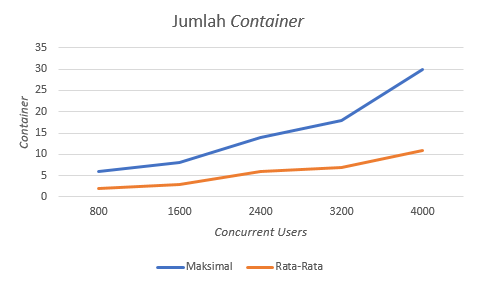
\includegraphics[width=8.7cm,height=4.7cm]{Images/C-5/jumlahcontainer.png}
	\caption{Grafik Jumlah \textit{Container}}
	\label{gjumlahcontainer}
\end{figure}

\subsubsection{Kecepatan Menangani \textit{Request}}
Dari hasil uji coba kecepatan menangani \textit{request}, dapat dilihat pada Table \ref{kecepatanrequest} dalam satuan detik bahwa semakin banyak \textit{concurrent users}, semakin lama pula waktu yang diperlukan untuk menyeselaikannya. Request paling cepat ditangani dengan menggunakan prediksi ARIMA(4,1,0) dan paling lambat menggunakan ARIMA(1,1,0). Hal tersebut terjadi karena kurang bagusnya hasil prediksi yang dihasilkan oleh ARIMA(1,1,0) yang mana kadang hasil prediksinya terlalu rendah atau terlalu tinggi.
Dari hasil percobaan tersebut, dapat dilihat bahwa hampir semua \textit{request} dapat ditangani di bawah satu menit. Lalu grafik hasil uji coba perhitungan kecepatan menangani \textit{request} ditunjukkan pada Gambar \ref{grunningtime}.
\begin{longtable}{|p{0.22\textwidth}|p{0.10\textwidth}|p{0.10\textwidth}|p{0.10\textwidth}|p{0.10\textwidth}|p{0.10\textwidth}|}
	\caption{Kecepatan Menangani \textit{Request}} \label{kecepatanrequest} \\
	\hline
	& \textbf{800} & \textbf{1600} & \textbf{2400} & \textbf{3200} & \textbf{4000} \\ \hline
	\endfirsthead
	\caption[]{Kecepatan Menangani \textit{Request}} \\
	\hline
	& \textbf{800} & \textbf{1600} & \textbf{2400} & \textbf{3200} & \textbf{4000} \\ \hline
	\endhead
	\endfoot
	\endlastfoot
	
	ARIMA(1,1,0) & 34.167 & 43.286 & 48.143 & 63.857 & 62.286 \\ \hline
	ARIMA(2,1,0) & 27.429 & 38.571 & 44.143 & 42.143 & 57.857 \\ \hline
	ARIMA(3,1,0) & 32.429 & 36.000 & 38.429 & 41.571 & 43.857 \\ \hline
	ARIMA(4,1,0) & 24.857 & 31.571 & 34.429 & 42.143 & 52.714 \\ \hline
\end{longtable}

\begin{figure}[H]
	\centering
	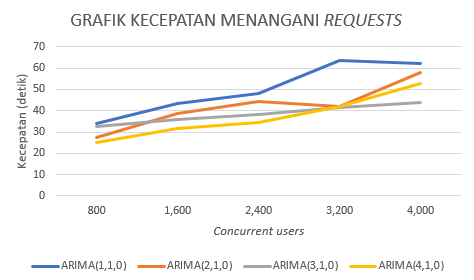
\includegraphics[width=8.7cm,height=4.7cm]{Images/C-5/runningtime.png}
	\caption{Grafik Kecepatan Menangani \textit{Request}}
	\label{grunningtime}
\end{figure}

\subsubsection{Penggunaan CPU}
Dari hasil uji coba penggunaan CPU pada \textit{server master host}, penggunaan CPU berada di bawah 15\%. Penggunaan CPU yang diukur adalah penggunaan CPU yang dilakukan oleh \textit{container} dari aplikasi, tidak termasuk sistem. Jumlah \textit{core} yang dimiliki oleh \textit{processor} di \textit{server master host} adalah 8 buah, yang artinya kurang lebih hanya satu core yang digunakan untuk menangani semua \textit{request}. Hasil pengukuran penggunaan CPU dapat dilihat pada Tabel \ref{penggunaancpu}

\begin{longtable}{|p{0.22\textwidth}|p{0.10\textwidth}|p{0.10\textwidth}|p{0.10\textwidth}|p{0.10\textwidth}|p{0.10\textwidth}|}
	\caption{Penggunaan CPU} \label{penggunaancpu} \\
	\hline
	& \textbf{800} & \textbf{1600} & \textbf{2400} & \textbf{3200} & \textbf{4000} \\ \hline
	\endfirsthead
	\caption[]{Penggunaan CPU} \\
	\hline
	& \textbf{800} & \textbf{1600} & \textbf{2400} & \textbf{3200} & \textbf{4000} \\ \hline
	\endhead
	\endfoot
	\endlastfoot
	
	ARIMA(1,1,0) & 7.1\% & 7.8\% & 9.1\% & 10.5\% & 10.7\% \\ \hline
	ARIMA(2,1,0) & 8.5\% & 9.2\% & 10.1\% & 11.3\% & 10.7\% \\ \hline
	ARIMA(3,1,0) & 8.8\% & 10.2\% & 11.6\% & 12.1\% & 10.3\% \\ \hline
	ARIMA(4,1,0) & 8.0\% & 8.3\% & 10.1\% & 12.9\% & 10.5\% \\ \hline
	
\end{longtable}

Dari hasil uji coba, penggunaan prediksi yang berbeda tidak terlalu berpengaruh terhadap penggunaan CPU. Lalu, penggunaan CPU tergolong rendah, yaitu hanya sebesar $\pm 10 \%$ untuk menangani semua \textit{request} yang diberikan. Hasil uji coba performa penggunaan CPU ditunjukkan oleh dalam grafik pada Gambar \ref{gcpuusage}.

\begin{figure}[H]
	\centering
	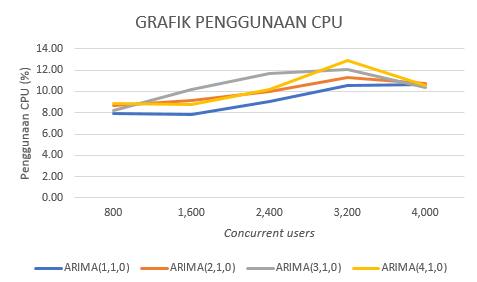
\includegraphics[width=8.7cm,height=4.7cm]{Images/C-5/cpuusage.png}
	\caption{Grafik Penggunaan CPU}
	\label{gcpuusage}
\end{figure}

\subsubsection{Penggunaan \textit{Memory}}            
Dari hasil uji coba penggunaan \textit{memory}, semakin banyak \textit{request} yang diterima, semakin banyak \textit{memory} yang diperlukan. Perhitungan penggunaan \textit{memory} adalah rata-rata penggunaan dari masing-masing \textit{container} sebuah aplikasi. Untuk masing-masing \textit{container}, dibatasi penggunaan maksimal \textit{memory} adalah 512 MB. Dari hasil uji coba ini, dapat dilihat pada Tabel \ref{penggunaanmemory} bahwa penggunaan terbesar hanya sebesar 158.71 MB. Artinya jumlah tersebut hanya menggunakan sepertiga dari keseluruhan \textit{memory} yang bisa digunakan.
\begin{longtable}{|p{0.22\textwidth}|p{0.10\textwidth}|p{0.10\textwidth}|p{0.10\textwidth}|p{0.10\textwidth}|p{0.10\textwidth}|}
	\caption{Penggunaan \textit{Memory}} \label{penggunaanmemory} \\
	\hline
	& \textbf{800} & \textbf{1600} & \textbf{2400} & \textbf{3200} & \textbf{4000} \\ \hline
	\endfirsthead
	\caption[]{Penggunaan \textit{Memory}} \\
	\hline
	& \textbf{800} & \textbf{1600} & \textbf{2400} & \textbf{3200} & \textbf{4000} \\ \hline
	\endhead
	\endfoot
	\endlastfoot
	
	ARIMA(1,1,0) & 67.91 & 88.97 & 130.79 & 120.14 & 157.73 \\ \hline
	ARIMA(2,1,0) & 65.89 & 97.98 & 123.47 & 156.64 & 158.33 \\ \hline
	ARIMA(3,1,0) & 72.20 & 99.72 & 125.56 & 144.42 & 152.14 \\ \hline
	ARIMA(4,1,0) & 69.60 & 77.34 & 117.39 & 149.76 & 158.71 \\ \hline
	
\end{longtable}

Hasil uji coba performa penggunaan \textit{memory} dalam grafik ditunjukkan pada Gambar \ref{gmemoryusage}.

\begin{figure}[H]
	\centering
	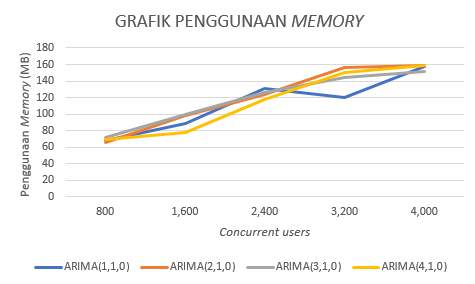
\includegraphics[width=8.7cm,height=4.7cm]{Images/C-5/memoryusage.png}
	\caption{Grafik Penggunaan Memory}
	\label{gmemoryusage}
\end{figure}

\subsubsection{Keberhasilan \textit{Request}}
Pada uji coba ini, dilakukan perhitungan seberapa besar jumlah \textit{request} yang gagal dilakukan. Untuk jumlah \textit{concurrent user} pada tingkat 800 dan 1600, dapat dilihat pada Table \ref{keberhasilanrequest} \textit{error} yang terjadi hampir sama. Prediksi menggunakan ARIMA(4,1,0) berhasil unggul karena menggunakan parameter yang lebih banyak. Namun hal tersebut tidak berlaku untuk ARIMA(3,1,0) karena walaupun parameternya lebih banyak dari ARIMA(2,1,0), tapi hasil prediksinya bisa meleset saat terjadi kondisi dimana koefisien negatif atau koefisien ke dua dikalikan dengan sebuah parameter bukan nol, dan koefisien lain dikalikan dengan parameter nol, maka hasil prediksinya akan negatif, yang mana seharusnya tidak mungkin ada \textit{request} negatif.
\begin{longtable}{|p{0.22\textwidth}|p{0.10\textwidth}|p{0.10\textwidth}|p{0.10\textwidth}|p{0.10\textwidth}|p{0.10\textwidth}|}
	\caption{\textit{Error Ratio Request}} \label{keberhasilanrequest} \\
	\hline
	& \textbf{800} & \textbf{1600} & \textbf{2400} & \textbf{3200} & \textbf{4000} \\ \hline
	\endfirsthead
	\caption[]{\textit{Error Ratio Request}} \\
	\hline
	& \textbf{800} & \textbf{1600} & \textbf{2400} & \textbf{3200} & \textbf{4000} \\ \hline
	\endhead
	\endfoot
	\endlastfoot
	
	ARIMA(1,1,0) & 5.72\% & 8.96\% & 12.85\% & 12.54\% & 13.38\% \\ \hline
	ARIMA(2,1,0) & 4.31\% & 9.35\% & 10.68\% & 8.11\% & 9.04\% \\ \hline
	ARIMA(3,1,0) & 4.84\% & 10.02\% & 13.22\% & 8.63\% & 12.24\% \\ \hline
	ARIMA(4,1,0) & 4.62\% & 8.41\% & 9.39\% & 7.52\% & 9.21\% \\ \hline
\end{longtable}

\begin{figure}[H]
	\centering
	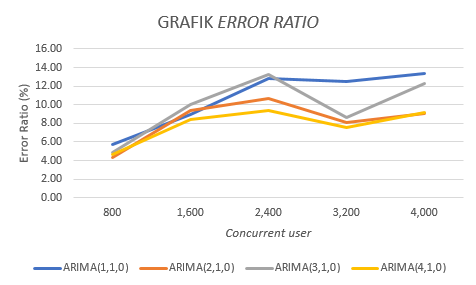
\includegraphics[width=8.7cm,height=4.4cm]{Images/C-5/errorratio.png}
	\caption{Grafik Error Ratio}
	\label{gerrorratio}
\end{figure}
Dari uji coba itu, 90\% lebih \textit{request} berhasil ditangani. Hasil uji coba jumlah \textit{request} yang gagal ditunjukkan dengan grafik pada Gambar \ref{gerrorratio}.